\documentclass[a4paper,10pt,twocolumn]{article}
\usepackage[utf8]{inputenc}
%\usepackage[francais]{babel}
\usepackage[T1]{fontenc}
\usepackage{graphicx}
\usepackage{eurosym}
\usepackage{verbatim}
\usepackage{amsmath, amsthm}
\usepackage{latexsym}
\usepackage{amssymb}
\usepackage{tabularx}
\usepackage{setspace}
\usepackage{listings}
\usepackage{geometry}
\usepackage{fancyhdr}
%\usepackage{enumitem}
\usepackage{colortbl}
%\usepackage[dvipsnames]{xcolor}
\usepackage{booktabs}
%\usepackage{moreverb}

%\usepackage{cite}
\DeclareMathAlphabet{\mathonebb}{U}{bbold}{m}{n}
\newcommand{\one}{\ensuremath{\mathonebb{1}}}

\usepackage{color}
%\usepackage{multirow}
%\usepackage{float}
\definecolor{gris25}{gray}{0.75}
\usepackage{colortbl}
\usepackage{fancyhdr}
\usepackage{amsmath,amsfonts,amssymb}
%\usepackage{titlesec}
%\usepackage{supertabular}
\usepackage{longtable}

\usepackage{caption}
\usepackage{subcaption}


\usepackage{listings}
\definecolor{dkgreen}{rgb}{0,0.4,0}
\definecolor{gray}{rgb}{0.5,0.5,0.5}
\definecolor{mauve}{rgb}{0.58,0,0.82}


\usepackage[numbers]{natbib}

\newcommand\Mycite[1]{%
  \citeauthor{#1}~(\citeyear{#1})~\cite{#1}}


\usepackage{multicol}
\usepackage{flushend}
\usepackage{balance}

%\usepackage{algorithm2e}

% marges,etc.
%\usepackage{a4wide}
\hoffset -2cm
\voffset -3cm
\textheight 27cm
\headheight 1cm
\headsep 1cm
\topmargin 0cm
\textwidth 19cm

%to change temporaly a margin
\def\changemargin#1#2{\list{}{\rightmargin#2\leftmargin#1}\item[]}
\let\endchangemargin=\endlist 


%pour les couleurs
\usepackage{color}
\definecolor{mycolor}{rgb}{0.06,0.32,0.39}

%liens dans le corps du texte
\usepackage{hyperref}
\hypersetup{
    colorlinks=true,
    linkcolor=blue,
    citecolor=dkgreen,
    filecolor=blue,
    urlcolor=blue,
}

\urlstyle{same}

\definecolor{dkyellow}{cmyk}{0, 0, 0.2, 0}
\lstset{
  language=Python,                % the language of the code
  basicstyle= \footnotesize,      % the size of the fonts that are used for the code
  numbers=left,                   % where to put the line-numbers
  numberstyle=\tiny\color{gray},  % the style that is used for the line-numbers
  stepnumber=2,                   % the step between two line-numbers. If it's 1, each line
                                  % will be numbered
  showspaces=false,               % show spaces adding particular underscores
  showtabs=false,                 % show tabs within strings adding particular underscores
  frame=single,                   % adds a frame around the code
  rulecolor=\color{black},        % if not set, the frame-color may be changed on line-breaks within not-black text (e.g. commens (green here))
  tabsize=2,                      % sets default tabsize to 2 spaces
  captionpos=b,                   % sets the caption-position to bottom
  breaklines=true,                % sets automatic line breaking
  breakatwhitespace=false,        % sets if automatic breaks should only happen at whitespace
  keywordstyle=\color{blue},      % keyword style
  commentstyle=\color{dkgreen},   % comment style
  stringstyle=\color{mauve},       % string literal style
  backgroundcolor=\color{white},      % choose the background color. You must add \usepackage{color}
}

\usepackage{array}
\newcolumntype{L}[1]{>{\raggedright\let\newline\\\arraybackslash\hspace{0pt}}m{#1}}
\newcolumntype{C}[1]{>{\centering\let\newline\\\arraybackslash\hspace{0pt}}m{#1}}
\newcolumntype{R}[1]{>{\raggedleft\let\newline\\\arraybackslash\hspace{0pt}}m{#1}}

\usepackage{xcoffins}
\NewCoffin\tablecoffin
\NewDocumentCommand\Vcentre{m}
  {%
    \SetHorizontalCoffin\tablecoffin{#1}%
    \TypesetCoffin\tablecoffin[l,vc]%
  }
\usepackage{lastpage}
% mise en forme des en-têtes et pieds de page
\usepackage{fancyhdr}
    \rhead{\markright}
    \lfoot{\scriptsize{Peter NAYLOR - June, 2016}}
    \cfoot{\footnotesize Page \thepage\ of \pageref{LastPage}}
    \rfoot{ \scriptsize{1st year PhD report}}
    \renewcommand{\headrulewidth}{0.6pt}
    \renewcommand{\footrulewidth}{0.5pt}
    \makeatletter
         \def\headrule{{\if@fancyplain\let\headrulewidth\plainheadrulewidth\fi
              \color{mycolor}\hrule\@height\headrulewidth\@width\headwidth \vskip-\headrulewidth}}
         \def\footrule{{\if@fancyplain\let\footrulewidth\plainfootrulewidth\fi
              \vskip-\footruleskip\vskip-\footrulewidth
              \color{mycolor}\color{mycolor}\hrule\@width\headwidth\@height\footrulewidth\vskip\footruleskip}}
    \makeatother
\pagestyle{fancy}

\fancypagestyle{plain}{%
  \renewcommand{\headrulewidth}{0pt}%
  \fancyhf{}%
  \fancyfoot[C]{\footnotesize Page \thepage\ of \pageref{LastPage}}%
}

\begin{document}

\title{Towards image-based cancer signatures from histopathology data}


\author{Peter Naylor \\ {\small \textit{Supervisor:} Thomas Walter and Fabien Reyal.}}
%\thanks{I am currently doing my PhD thesis with the center of computational biology that is affiliated to Mines ParisTech and Institut Curie.}

\markboth{Annual activity report with respect to my 1st year of PhD}{}

\maketitle


%\begin{abstract}
%\boldmath
%\blindtext[1]
%\end{abstract}

The summary of this report is the following. I will start by giving a brief introduction of my PhD subject, continued with the main difficulties to overcome and a brief bibliography. A chronological assessment of my work follows: from November to April I worked on tissue segmentation, Nuclei segmentation is my current focus and I will conclude with my future work.

\section{PhD subject: objectives and strategy}

This  PhD  project aims at developing the tools to take advantage of
the morphological and spatial information at the cellular and tissular
scale from histopathology data. 

%is a first step in integrating morphological and
%phenotypic information at the cellular and tissular scale into a
%bioinformatics workflow. 

The basic work flow is shown in Figure \ref{workflow1}. Tissue samples
are taken from the breast prior to surgery. In parallel, slides are
prepared and the tissue is profiled in terms of gene expression and /
or sequencing. From the work flow, we aim at extracting physiologically
relevant features, which can then be used (optionally in combination with
expression and mutational data) to predict either the molecular
cancer subtype or the prognosis for the patient. 



The main focus of this PhD thesis will be the extraction of
physiologically relevant features at the cellular and tissue
level. Regarding the {\em cellular level}, I will focus on nuclear morphologies,
because (1) nuclei are indicative of many cellular
phenotypes\citep{Chow2012} and (2) their morphology is currently used by
pathologists in order to identify the mitotic index and the level of
nuclear pleomorphism\citep{Elston1991}. In order to derive information
at the cellular level, nuclei must first be identified by automatic
segmentation. Second, each of the segmented nuclei can be described
with respect to texture, color and shape in order to assign a cell
type to each of the nuclei (such as epithelial cell, stromal cell or
lymphocyte) by a supervised learning approach (using SVM or Random
Forests). Some of the features will also be exported directly, as they
are themselves physiologically relevant (such as cell size). 
Regarding the {\em tissue level}, the plan is to detect the tumor,
stromal and necrotic regions (regions containing mostly dead
cells). The tissue level features I will consider, are on the one hand
region based features, calculated on the regions, and on the other
hand features calculated from the cell populations (such as cell type
percentages, and features describing the level of organization, such
as Ripley's K), stratified by the regions in which the cells are situated. 
In both cases, segmentation will be probably a bottleneck, and I am
particularly interested by methods that are easily adaptable to new
data sets and new segmentation tasks.

\paragraph{Data sets}

I will apply these methods to
two datasets: (1) 208 slides from an unpublished study on breast
cancer, a special type of very aggressive breast cancer  and (2) 198
slides from a recently published study on bladder cancer
\citep{biton2014independent}. In the first data set, I will be able to
study the predictability of treatment response by automatic
analysis of histopathology data. The second data set will be
informative about how the histopathology features correlate with the
molecularly defined subgroups. Indeed, I hope to identify links between
cellular phenotypes, transcriptomic and grading data that will feed
future projects in this field with interesting hypotheses. 

In this PhD thesis, I want to contribute to the generation of the
appropriate tools to quantify the huge amount of data found in
histopathology slides. On the long run, such a
 quantification scheme would fit in a work pipeline that would
 investigate the most informative physiological features at the
 cellular and the tissue level and the links
 to genomic, transcriptomic features and even possibly different
 medical imaging such as 3D MRI scans. 

\section{Context and difficulties}

So far, histopathology data is still largely unexploited in a systematic and
quantitative way. There are several reasons for this: 

\begin{enumerate}
\item With the
availability of comprehensive genome, transcriptome and epigenome data
sets, the hope was that these data could explain many aspects of life
and virtually all aspects of diseases which are known to be related to
the genome. Today, we understand that it is necessary to include the spatial and
morphological dimensions in the reasoning. 
\item Digital pathology,
has only recently become a standard in the field. Still a few years
ago, the standard
procedure was to examine the slides on the
microscope. We now have powerful scanner that produce whole slide images.
\item The information
contained in histopathology data has never been fully
formalized. While some quantitative (yet manually determined) criteria
exist, this is not true for the overall interpretation of slides
which remains subjective and difficult to model formally. This issue is also linked with the high variability between slides, which is due to the stain variability between and the tissue variability. 
\item There are many technical and methodological challenges related
  to the automatic analysis of histopathology data which made fully
  automated analysis of these images unfeasible. In particular, we can think of the size of the data, more then $50GB$ per slide and we have hundreds of slides.
\end{enumerate}
However, many people have started to work on histopathology slides, these works try to cope
 with these difficulties and our often focused on the detection of objects within histopathology slides. More recent work 
 have started analysing correlations, and some times it's complementation with respect to 
 other data types. Image-based biological features are also emerging: In \citet{lee2015supervised}, 
 they improve the prediction of recurrent prostate cancer via the integration of quantitative 
 image features and protein expression. 
% \citet{yuan2012quantitative} segment nuclei in 
% histological data to access information about lymphocyte counts, cancer cells counts and 
% heat maps of spatial distribution in order to model prediction.  They also use these biological 
% driven features to correct statistical models based on molecular data, indeed they assess that  
% these biologic driven features quantify the heterogeneous cell populations that is a source of 
% noise. 
 Evaluating tumor heterogenity is an important aspect, in \citet{potts2012evaluating} 
 they quantify cell heterogeneity in two ways, intratumoral, linked to the variability of cells 
 within a tumor, and intertumoral which is linked to tumor heterogeneity within the whole 
 tissue. They increase the accuracy of HER2 scoring by better quantifying the heterogeneity 
 via features based on spatial distribution and local neighbourhoods. 
 \citet{harder2016cooccurence} find relevant biological features that quantify the invasion of 
 the tumor, in particular these features are based on spatial and neighbourhood analysis. In 
 \citet{petushi2006large}, they show that we can extract relevant data from the images in 
 order to create reproducible grading. Reproducibility of the grading is a key goal for computer 
 aided diagnostics, indeed breast cancer grading and many others can be highly variable from 
 one pathologist to another, even from one hospital to another, this issue can be seen in the 
 figures \ref{fig:example_histopath}. 

\section{Tissue segmentation}

Histopathology annotated data is very scarce, indeed, whole slide images (WSI) are very large files that need expert pathologist in order to highlight the relevant information. Camelyon16, a challenge covered by ISBI2016, offered an ideal dataset. We had 270 annotated WSI provided by two different hospital, every metastasis region in this data set was annotated, see figure \ref{fig:AnnotatedData}. To gain a first insight in histopathology, large image files and computer vision, I trained a supervised model based on hand crafted features in order to try and predict metastatic regions. These hand crafted features were based on two distinct methods: some were extracted from the software \textit{Ilastik}, these features were the result of the application of image filters at different scales, gaussian smoothing, Laplacian of Gaussian, etc. Others were extracted via the use of mathematical morphology and in particular  waterpixels, \citep{waterpixels}. The work flow for the feature extraction can be found in figure \ref{fig:workflowCAM}. Once we had the features we applied a random forest tuned via cross validation. The training was a delicate part as the data set was huge and highly unbalanced, more than $5 . 10^{12}$ lines and only $1\%$ were positive. We used a modified random forest in order to speed up convergence, the sampling procedure was modified in order to reduce the computational burden. We presented a unique part of the data set to each tree construction instead of the whole dataset, see \citep{breiman}. This novel random forest wasn't any less accurate then the standard random forest, however the speed up was considerable. From this classifier we were able to produce heat maps, see figure \ref{fig:output}. 

Our results were unsatisfying as our heat maps were very noisy and our classifier did not seem to pick up on the highly variable metastatic regions. We think that our features were not adapted for such a high variable task, indeed none of the top submitters to this challenge used hand crafted features, however they used deep networks and in particular deep convolutionnal network such Image Net \citep{ImageNet} and GoogleNet \citep{szegedy2015going}. The results achieved were astonishing and they have set us on a new segmentation task, nuclei segmentation within histopathology slides.

\section{Nuclei segmentation}

Nuclei segmentation annotation for histopathology is an even scarcer dataset, the number of
 cells in one histopathology slide could reach millions of cells. The work flow for this part is
 pictured in figure \ref{fig:ComputerVision}. In order to apply supervised classifiers we started
 creating our own manual annotation for a limited number of patches of the slides. In order to 
 help the workload, we used a previous unsupervised segmentation approach to do a first 
 segmentation, if this first segmentation is too poor we discard it, if not we correct it and save 
 the patch. The software used for the manual segmentation is \textit{itksnap}. Once we have 
 sufficient annotation samples we will be able to train, or \textit{fine-tune} our network. We 
 will be using fully convolutional network for their state of the art semantic segmentation on  
 Image net \citep{long2015fcn} and in medical imaging, \citep{UNet}. Once the segmentation over the 
 whole slide is achieved, we can consider extracting object specific features in order to classify 
 each nuclei with respect to his type  (lymphocyte, epithelial cell, cancerous cell and so on) but 
 also to his current state (undergoing mitosis, apoptosis and so on). Thank to this classification we can create density maps over the slide and create other biological relevant features, such as lymphocyte density counts and maybe spatial distribution features. The relevance of such features have been shown in recent works \cite{yuan2012quantitative, lee2015supervised}. 
 
 
 Once the nuclei segmentation step achieved, we will be able to use the information provided by the density counts in order to derive more information about the tissues, for instance detecting metastatic regions, necrotic tissue and healthy tissue. All the information gathered on one WSI will be summed up as a highly dimensional feature vector that will try and describe the histopathology data in a biologically relevant aspect for one patient.
 
 \section{Future work}
Once the computer vision aspect concluded, which is one of the bottlenecks for this PhD subject. We will focus on the different aspect present in figure \ref{workflow1}. In particular extracting features from the genomic data and combining the very heterogeneous data set is a difficult task. Indeed, even if the extraction procedure are independent, the data will stay highly dependent. We wish to explore links between genomic signatures and phenotypic patterns, exploring the links between these heterogeneous type of data will enable us to better exploit the present complementary information between them in order to increase the performance of only genomic models. Other works have investigated the combination of such heterogeneous type of data. As an example, \citet{yuan2012quantitative} segment nuclei in 
 histological data to access information about lymphocyte counts, cancer cells counts and 
 heat maps of spatial distribution in order to improve genomic based models.  They also use these biological 
 driven features to correct statistical models based on molecular data, indeed they assess that  
 these biologic driven features quantify the heterogeneous cell populations that is a source of 
 noise.
 
 \newpage
 

\section*{Appendix}

\bibliographystyle{plainnat}
%\bibliographystyle{abbrvnat}
{\footnotesize\bibliography{biblio.bib}
}


 \begin{figure*}[!ht]
\centering
\includegraphics[width=0.6\textwidth]{Workflow_overview.png}
\caption{Workflow}
\label{workflow1}
\end{figure*}


\begin{figure*}[!ht]
\centering
\includegraphics[width=0.6\textwidth]{ComputerVision.png}
\caption{Computer Vision aspect}
\label{fig:ComputerVision}
\end{figure*}

\begin{figure*}[!ht]
\centering
\begin{subfigure}{.3\textwidth}
  \centering
  \includegraphics[height=3cm]{histo1.png}
  \caption{}
  \label{fig:sub1}
\end{subfigure}%
~
\begin{subfigure}{.3\textwidth}
  \centering
  \includegraphics[height=3cm]{histo2.png}
  \caption{}
  \label{fig:sub2}
\end{subfigure}
~
\begin{subfigure}{.3\textwidth}
  \centering
  \includegraphics[height=3cm]{histo3.png}
  \caption{}
  \label{fig:sub3}
\end{subfigure}
\caption{Tissue sections with standard Haematoxylin and Eosin staining.}
\label{fig:example_histopath}
\end{figure*}

\begin{figure*}[!ht]
\centering
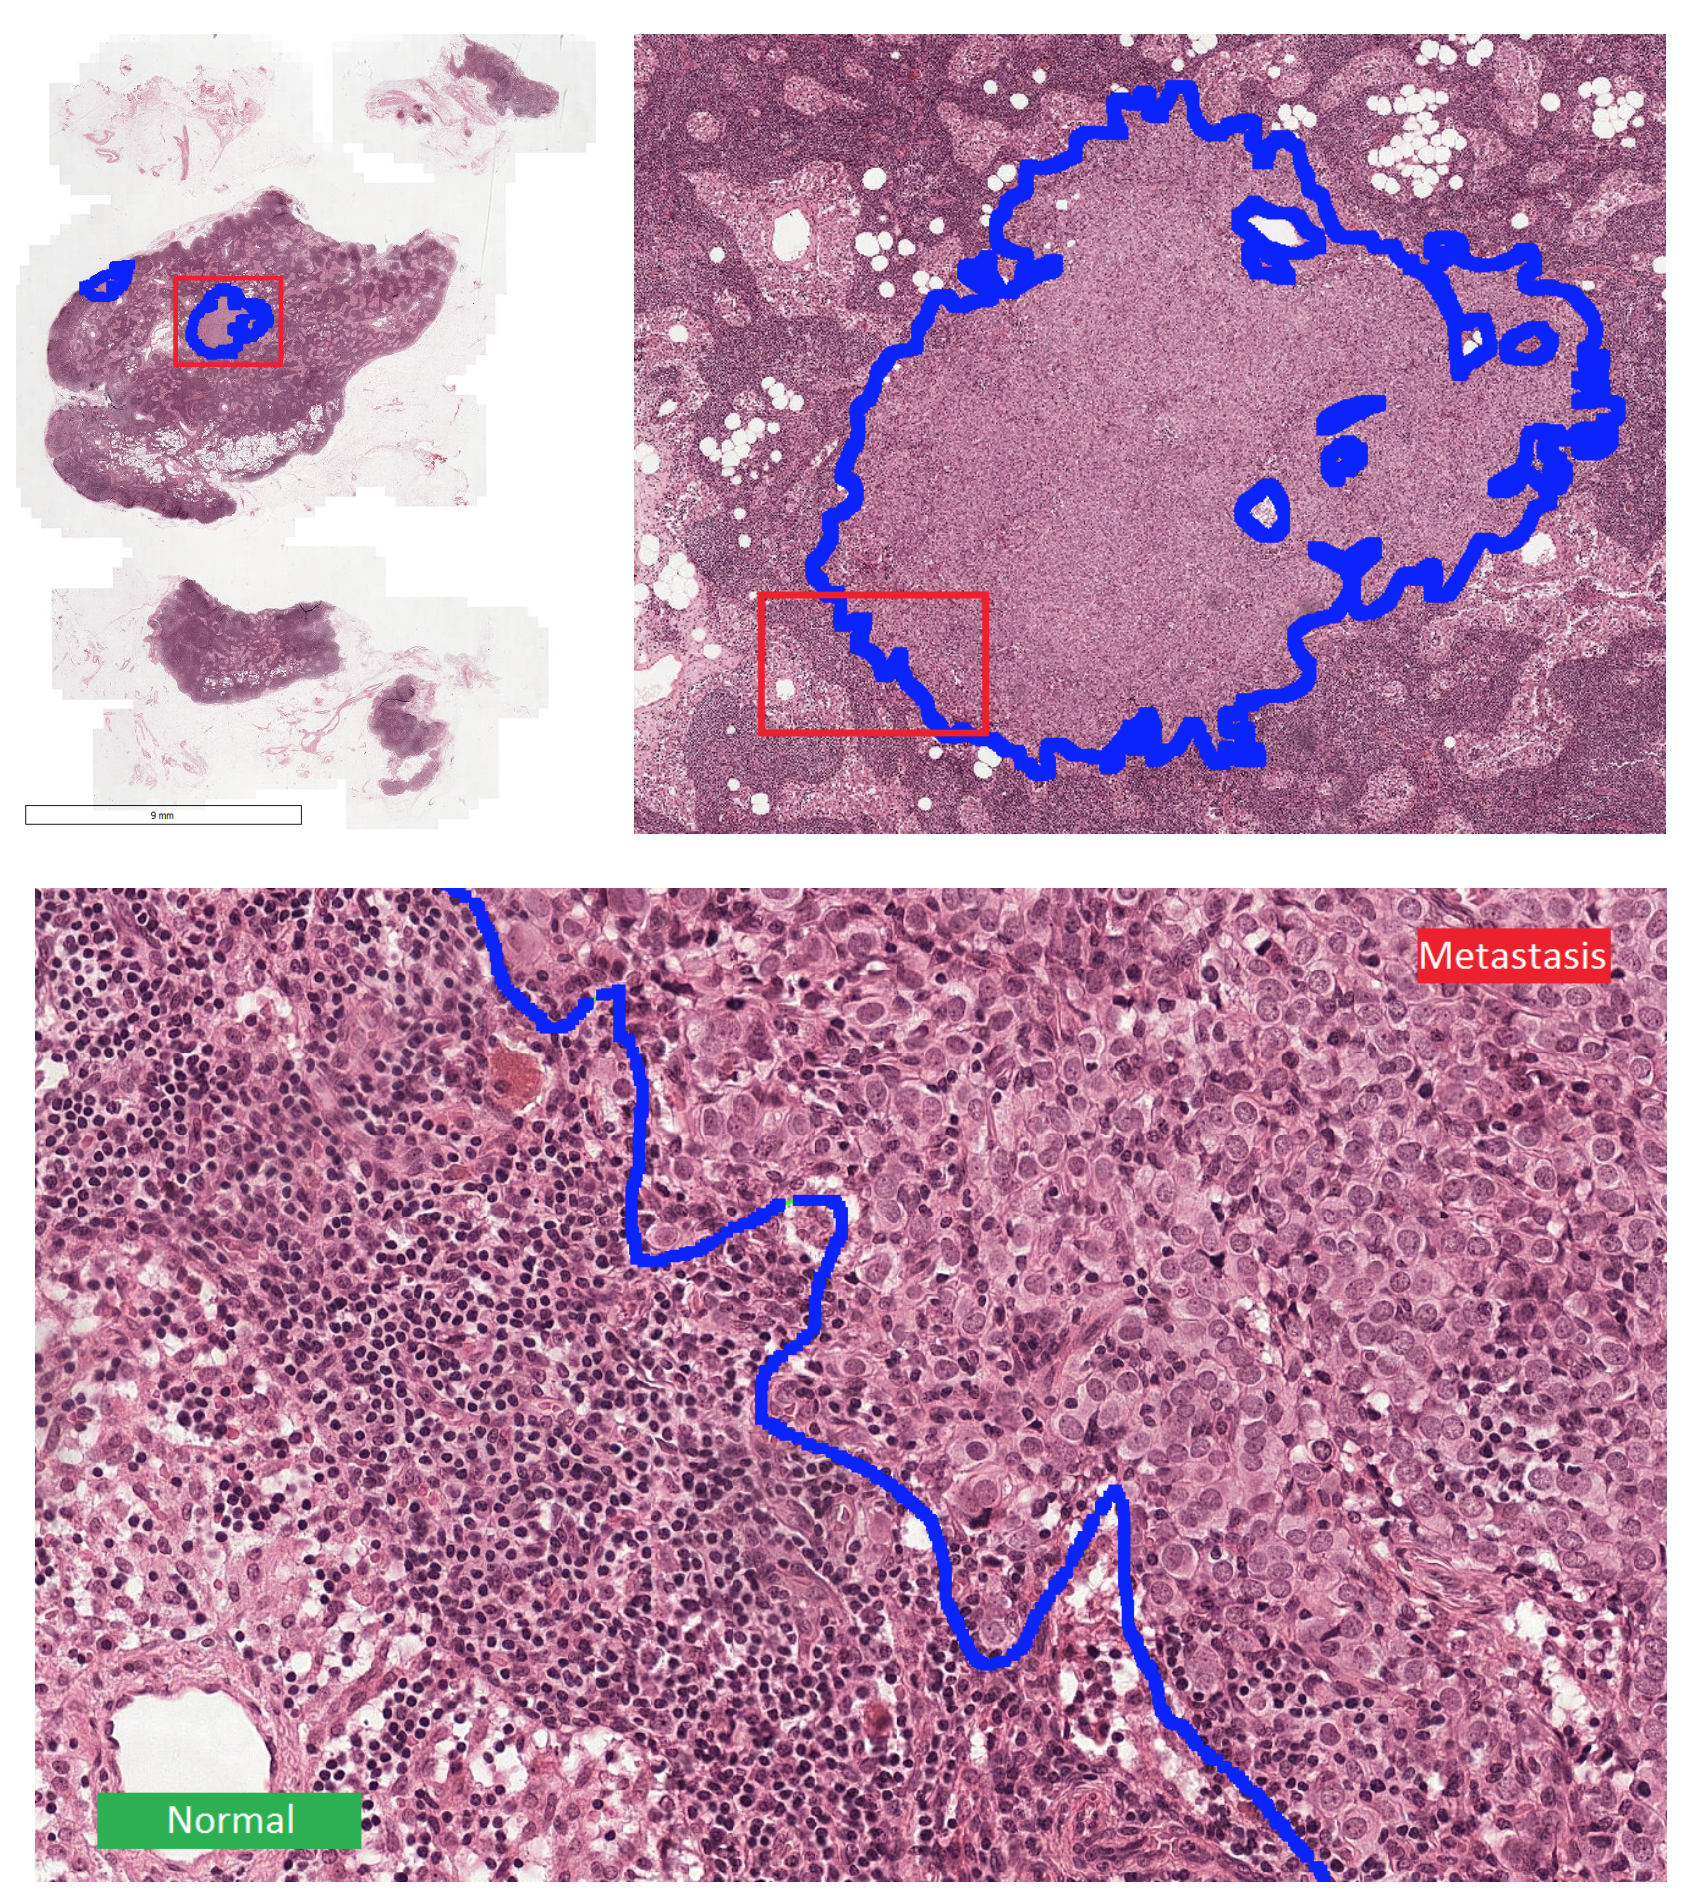
\includegraphics[width=0.4\textwidth]{AnnotatedData.png}
\caption{Annotated data}
\label{fig:AnnotatedData}
\end{figure*}

\begin{figure*}[!ht]
\centering
\includegraphics[width=0.7\textwidth]{workflowWithoutMil.png}
\caption{Work flow for metastatic region detection}
\label{fig:workflowCAM}
\end{figure*}
%\twocolumn
\begin{figure*}[!ht]
\centering
\begin{subfigure}{.33\textwidth}
  \centering
  \includegraphics[height=6cm]{Test_002_whole.png}
  \caption{RGB raw data.}
  \label{RawImage}
\end{subfigure}%
\begin{subfigure}{.33\textwidth}
  \centering
  \includegraphics[height=6cm]{whole_probmap_Test_002.png}
  \caption{Probability map.}
  \label{ProbabilityMapLocalMaxima}
\end{subfigure}
\begin{subfigure}{.33\textwidth}
  \centering
  \includegraphics[height=6cm]{Detection.png}
  \caption{Metastasis confidence pin-points.}
  \label{Detecting maxima}
\end{subfigure}
\textit{For figure (c), blue is equal to a low confidence score whereas red means a high confidence.}
\caption{Evaluation whole slide image, test slide number 2.}
\label{fig:output}
\end{figure*}






\end{document}